\section{Sistema de Monitoreo Ambiental}

\begin{table}[H]
	\centering
	\begin{tabular}{llrrrr} \hline
		\textbf{Ciudad}          & \textbf{Nombre} & \textbf{Elevación} & \textbf{Latitud} & \textbf{Longitud} \\ \hline
		Guadalupe                & Sureste         & 492                & 25.6680          & -100.2490         \\
		Monterrey                & Centro          & 560                & 25.6700          & -100.3380         \\
		Monterrey                & Noroeste        & 571                & 25.7570          & -100.3660         \\
		San Nicolas de los Garza & Noreste         & 476                & 25.7500          & -100.2550         \\
		Santa Catarina           & Suroeste        & 694                & 25.6760          & -100.4640         \\
		Garcia                   & Noroeste2       & 716                & 25.7830          & -100.5860         \\
		Escobedo                 & Norte           & 528                & 25.8000          & -100.3440         \\
		Apodaca                  & Noreste2        & 432                & 25.7770          & -100.1880         \\
		Juarez                   & Sureste2        & 387                & 25.6460          & -100.0960         \\
		San Pedro Garza Garcia   & Suroeste2       & 636                & 25.6650          & -100.4130         \\
		Cadereyta de Jimenez     & Sureste         & 340                & 25.3600          & -99.9955          \\
		Monterrey                & Sur             & 630                & 25.5749          & -100.2489         \\
		San Nicolas de los Garza & Norte2          & 520                & 25.7295          & -100.3099         \\ \hline
	\end{tabular}
	\caption{}
	\label{table:stations_information}
\end{table}


\subsection{Limpieza de datos}
\subsection{Reconstrucción}
\section{Creación de la base de datos}
\subsection{Condiciones de cielo despejado}

A partir de las graficas diarias de la medición con los modelos, se centraron algunas mediciones con respecto al máximo solar, esto debido a que en algunas estaciones ocurria este error de forma esporpádica. Existian mediciones en los datos los cuales son imposibles físicamente, para ello se realizo una limpieza automatica de los datos. Esta limpieza consistia en eliminar aquellos valores que tuvieran una diferencia negativa con respecto al modelo GHI$_0$ o tuvieran una valor de k$_t$ (GHI/GHI$_0$) mayor a 0.8. Cuando el valor del modelo GHI$_0$ es 0 para una hora, este valor sera remplazado independientemente del criterio anterior. Esto debido a que representa un valor con ruido. Al termino de la limpieza, el tratamiento de los datos se enfoco en realizar una restauración de los mismos. Para ello se hizo uso de la similitud coseno (ecuación \ref{eq:cosine}).


\begin{equation}
	sim(m_i , m_j ) = \frac{m_i \cdot m_j}{||m_i|| ||m_j||}
	\label{eq:cosine}
\end{equation}

Se calculo la similitud coseno para mediciones de la misma estación, esto debido a que la topología alredor de cada una de ellas es diferente y esto puede ocasionar que existe una irregularidad si se toman todas a la vez. Para cada día se seleccionaron las primeras 30 mediciones que tuvieran una similitud más cercana a 1. Con estas mediciones seleccionadas se calculo el promedio horario, para así restaurar la mediciones con datos faltantes. En la figura \ref{fig:restoration} se muestran casos de restauración de datos en diferentes estaciones y días.

\begin{figure}[H]
	\centering
	\begin{subfigure}{15cm}
		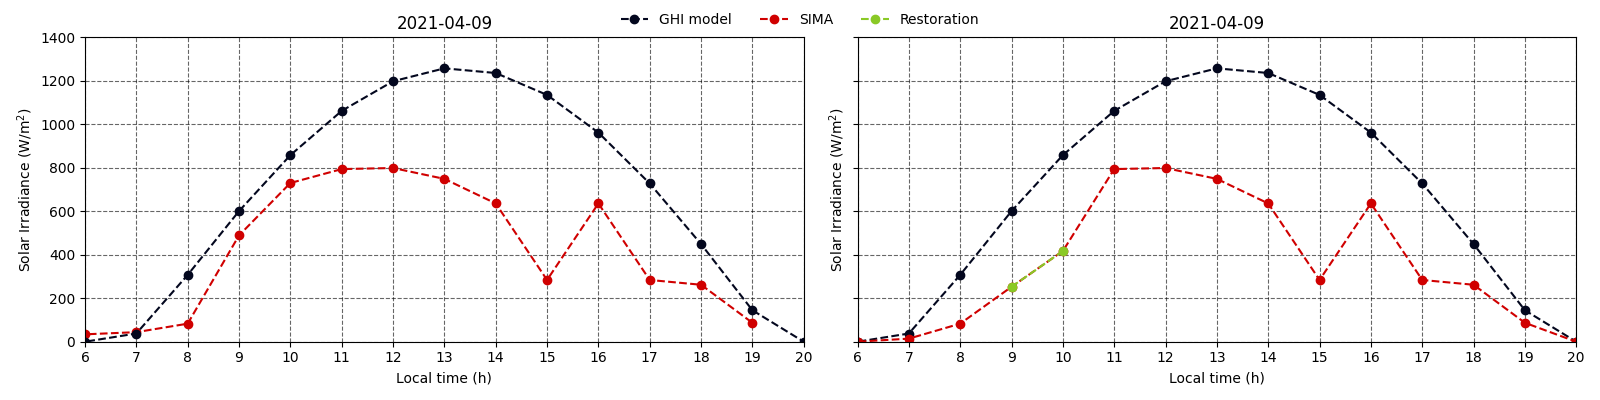
\includegraphics[width=15cm]{Graphics/2021-04-09.png}
	\end{subfigure}
	\begin{subfigure}{15cm}
		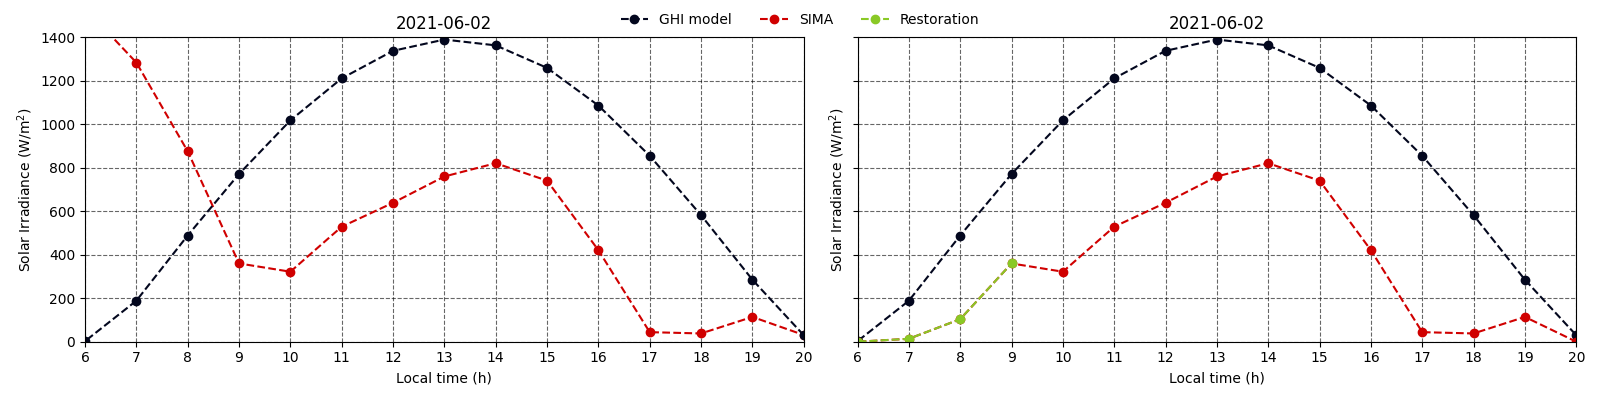
\includegraphics[width=15cm]{Graphics/2021-06-02.png}
	\end{subfigure}
	\begin{subfigure}{15cm}
		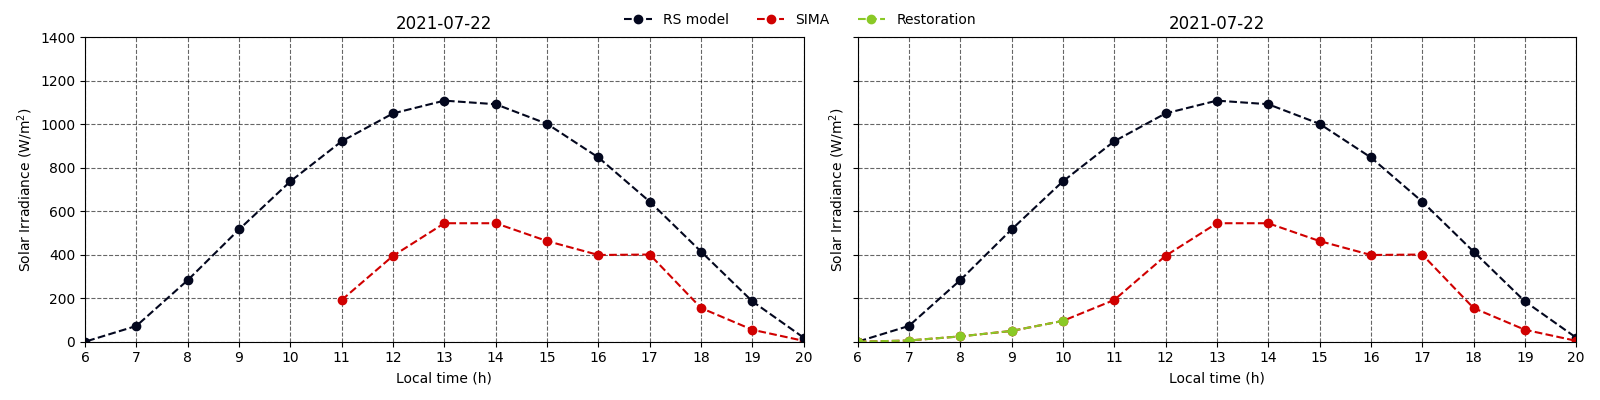
\includegraphics[width=15cm]{Graphics/2021-07-22.png}
	\end{subfigure}
	\begin{subfigure}{15cm}
		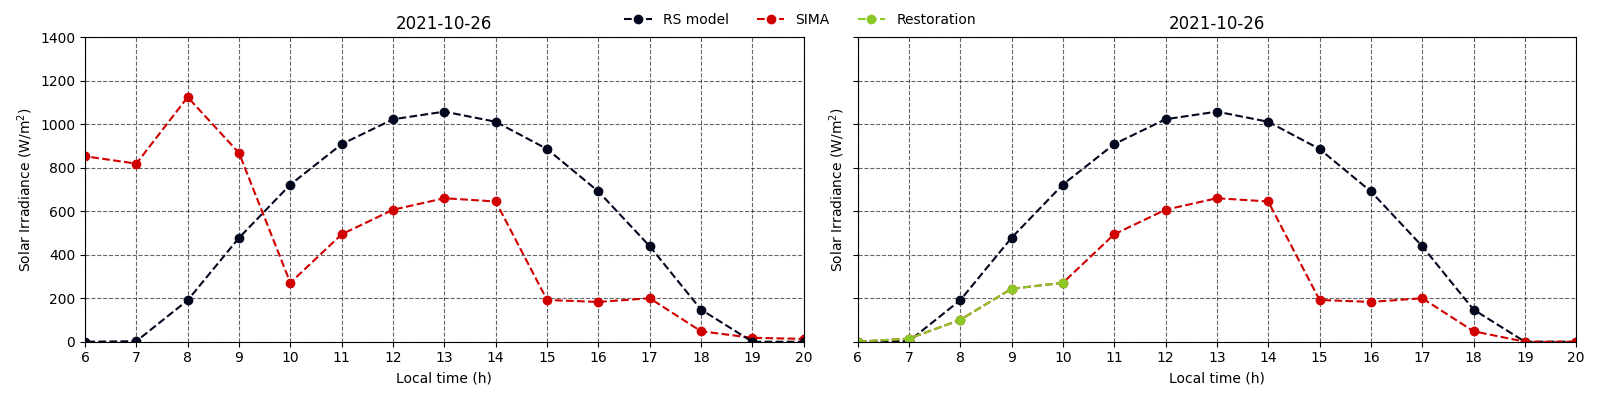
\includegraphics[width=15cm]{Graphics/2021-10-26.png}
	\end{subfigure}
	\caption{Restauracion de mediciones por medio de promerios horarios de las 30 mediciones más semejantes al día seleccioando}
	\label{fig:restoration}
\end{figure}

Con las mediciones restauradas se realizaron las comparaciones (diferencias y razones) con respecto a los modelos (GHI$_0$ y RS). Estas comparaciones seran usadas para entrenar a los modelos de clasificación clasicos y basados en redes neuronales.
